\documentclass[12pt]{beamer}

\usepackage[T1]{fontenc}
\usepackage[utf8]{inputenc}
\usepackage{graphicx, tikz-qtree, caption, chronology}

\usetheme{CambridgeUS}
\usecolortheme{seagull}
\setbeamertemplate{title page}[default][shadow=false]
\setbeamertemplate{headline}{}
\setbeamertemplate{itemize items}[triangle]
\setbeamertemplate{footline}[frame number]{}
\setbeamertemplate{navigation symbols}{}

\title{Esquemas de assinatura digital \\ pós-quânticos baseados em AES}
\author{Gustavo Zambonin\and Marcello Klingelfus}
\institute{
  
\includegraphics[scale=0.15]{ufsc}            \\ \vspace{-4mm}
  Universidade Federal de Santa Catarina        \\
  Departmento de Informática e Estatística      \\ \vspace{2mm}
  \texttt{\{gustavo.zambonin,marcello.klingelfus\}@grad.ufsc.br}
}
\date{}

\newcommand{\concat}{\, \vert \vert \,}
\newcommand{\hh}{$\mathcal{H}$}
\newcommand{\hash}[2][]{\mathcal{H}^{#1}(#2)}
\newcommand{\pad}{\vert \vert \, 0^*}

\begin{document}

\begin{frame}[plain,noframenumbering]
  \titlepage
\end{frame}

\begin{frame}
  \frametitle{Motivação}
  \begin{itemize}
    \setlength\itemsep{0.5em}
    \item Independente de teoria de números ou problemas algébricos
    \begin{itemize}
      \item Possivelmente ``seguro contra computadores quânticos''
    \end{itemize}
    \item Para um esquema de assinatura digital, qualquer função
        de resumo criptográfico pode ser utilizada
    \begin{itemize}
      \item Escolhida situacionalmente (hardware, software)
    \end{itemize}
    \item Funções de mão única são necessárias e suficientes para assinatura digital
      \cite{Rompel:1990:OFN:100216.100269, cryptoeprint:2005:328}
    \item Cifras de bloco podem ser utilizadas na construção de funções de mão única
  \end{itemize}
\end{frame}

\begin{frame}
  \frametitle{Fundamentação}
  \framesubtitle{Funções de resumo criptográfico}
  \begin{equation*}
    \mathcal{H}: \{0, 1\}^{*} \longrightarrow \{0, 1\}^{n}
  \end{equation*}

  \begin{figure}
    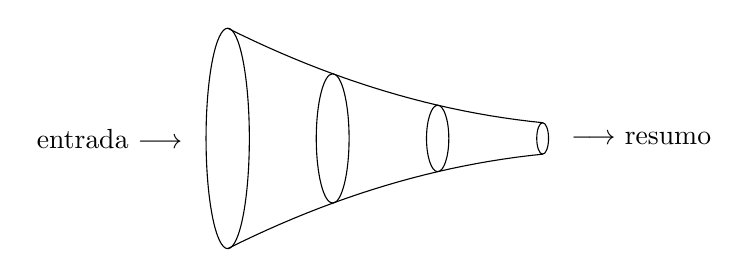
\begin{tikzpicture}
      \node at (-6.5, 0) {entrada $\longrightarrow$};
      \foreach \sgn in {+, -}
        \draw plot[domain=1:5] (-\x, {\sgn 1/20*(3+\x*\x)});
      \foreach \r in {1, 2.3333, ..., 5}
        \draw (-\r, 0) ellipse[x radius=(\r+.5)/20, y radius=1/20*(3+\r*\r)];
      \node at (0.25, 0) {$\longrightarrow$ resumo};
    \end{tikzpicture}
  \end{figure}

  \begin{itemize}
    \item SHA-2, SHA-3, BLAKE: $n \in \{224, 256, 384, 512\}$
    \item Keccak: qualquer $n$
    \item Resistência à pré-imagem, segunda pré-imagem, colisão
  \end{itemize}
\end{frame}

\begin{frame}
  \frametitle{Assinaturas digitais}
  \begin{itemize}
    \item Provêm autenticação, integridade e não-repúdio
    \item Baseado em criptografia de chaves públicas
    \item Tripla de algoritmos probabilísticos de tempo polinomial
      \cite{Goldreich:2004:FCV:975541}
    \begin{itemize}
      \item Geração de chaves (\emph{Gen}), geração da assinatura (\emph{Sig}),\\
          verificação da assinatura (\emph{Ver})
    \end{itemize}
  \end{itemize}

    \begin{figure}[h]
      \centering
      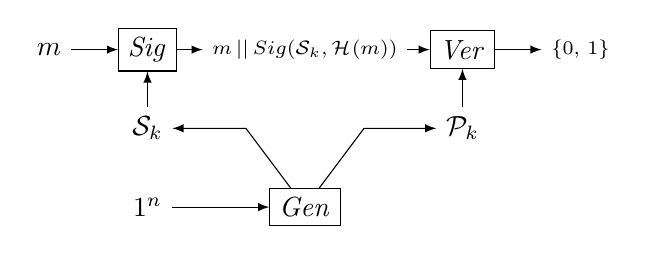
\begin{tikzpicture}
        \node (hm) at (-1.25, 0) {$m$};
        \node (in) at (0, -2) {$1^n$};
        \node (sk) at (0, -1) {$\mathcal{S}_k$};
        \node (pk) at (4, -1) {$\mathcal{P}_k$};
        \node (ds) at (2, 0)
          {\scriptsize{$m \concat Sig(\mathcal{S}_k, \hash{m})$}};
        \node (res) at (5.5, 0) {\scriptsize\{0, 1\}};
        \node[draw] (sig) at (0, 0) {\emph{Sig}};
        \node[draw] (gen) at (2, -2) {\emph{Gen}};
        \node[draw] (ver) at (4, 0) {\emph{Ver}};
        \draw[-latex] (gen) to (1.25, -1) to (sk);
        \draw[-latex] (gen) to (2.75, -1) to (pk);
        \draw[-latex] (sk) -- (sig);
        \draw[-latex] (hm) -- (sig);
        \draw[-latex] (sig) -- (ds);
        \draw[-latex] (ds) -- (ver);
        \draw[-latex] (pk) -- (ver);
        \draw[-latex] (ver) -- (res);
        \draw[-latex] (in) -- (gen);
      \end{tikzpicture}
    \end{figure}
\end{frame}

\begin{frame}
    \frametitle{AES}
    \begin{itemize}
        \item Uma cifra de blocos simétrica e reversivel
        \item Suas operações são definidas sobre um corpo finito
        $\mathbb{F}_{2^{8}}$
        \item Sua chave tem tamanho $n = \{128,192,256 \}$
    \end{itemize}
    
\end{frame}

\begin{frame}
    \frametitle{AES}
    \framesubtitle{Funcionamento}
    \begin{itemize}
        \item Cada bloco é representado por uma matriz de estado $A$ de dimensões $4 \times 4$
        \item Seu funcionamento é constituido de multiplas iterações das seguintes operações em $A$, em relação a chave referente iteração a atual:
        \begin{itemize}
            \item\textsc{SubBytes}
            \item\textsc{ShiftRows}
            \item\textsc{MixColumns}
            \item\textsc{AddRoundKey}
        \end{itemize}
        \item A chave utilizada em cada iteração é obtida através de uma rotina de expansão da chave, denominada \textsc{KeyExpansion}
    \end{itemize}
\end{frame}

\begin{frame}
    \frametitle{AES}
    \framesubtitle{Operações}
    
\end{frame}

\begin{frame}
  \frametitle{One-time signature schemes}
  \begin{itemize}
    \item Par de chaves só deve ser utilizado uma única vez
    \item Lamport-Diffie (LD-OTS)
    \begin{itemize}
      \item Primeiro esquema baseado em resumos
      \item Mensagens de tamanho arbitrário podem ser assinadas, um bit por vez
    \end{itemize}
    \item Winternitz (WOTS)
    \begin{itemize}
      \item Multiplos bits podem ser assinadas simultaneamente
      \item Generalização do LD-OTS
      \item Compensação entre a performance e o tamanho da assinatura
    \end{itemize}
    \item HORS
    \begin{itemize}
      \item Esquema de poucas vezes, segurança diminui a cada assinatura
      \item HORST --- HORS com árvores
    \end{itemize}
  \end{itemize}
\end{frame}

\begin{frame}
  \frametitle{Winternitz OTS}
  \framesubtitle{Generalização de chave}
  Seja $w \in \mathbb{N}, w > 1$ o parâmetro de compensação Winternitz. Entao,
   \begin{align*}
       t_1 &= \left\lceil \frac{n}{w} \right\rceil \\
       t_2 &= \left\lceil
       \frac{\lfloor log_2 t_1 \rfloor + 1 + w}{w} \right\rceil \\
         t &= t_1 + t_2
   \end{align*}
   As chaves privada e pública são, respectivamente,
   \begin{align*}
     S_k &= (y_{t - 1}, \dots, y_{0})
       \stackrel{\$}{\longleftarrow} \{0,1\}^n \\
     P_k &= (\hash[2^w - 1]{y_{t - 1}}, \dots, \hash[2^w - 1]{y_0})
   \end{align*}
\end{frame}

\begin{frame}
  \frametitle{Winternitz OTS}
  \framesubtitle{Assinatura}
  Os expoentes da cadeia de resumo $\epsilon_i \in \{0, 1\}^w$
  são produzidos através de:
  \begin{minipage}{.45\linewidth}
  \begin{align*}
    \hash{m} &= (\epsilon_{t - 1}, \dots, \epsilon_{t - t_1})
  \end{align*}
  \end{minipage}
  \begin{minipage}{.45\linewidth}
  \begin{align*}
    c &= \sum_{i = t - t_1}^{t - 1} (2^w - 1 - \epsilon_i) \\
      &= (\epsilon_{t_2 - 1}, \dots, \epsilon_{0})
  \end{align*}
  \end{minipage}
  \vspace{4mm}
  
  Finalmente, a assinatura de uso único é construida.
  \begin{align*}
    \sigma &= (\mathcal{H}^{\epsilon_{t - 1}}(y_{t - 1}),
    \dots, \mathcal{H}^{\epsilon_0}(y_0))
  \end{align*}
\end{frame}

\begin{frame}
  \frametitle{Winternitz OTS}
  \framesubtitle{Verificação}
  Lembre-se que
  \begin{align*}
    P_k &= (\hash[2^w - 1]{y_{t - 1}}, \dots, \hash[2^w - 1]{y_0}) \text{ e} \\
    \sigma &= (\mathcal{H}^{\epsilon_{t - 1}}(y_{t - 1}), \dots, \mathcal{H}^{\epsilon_0}(y_0))
  \end{align*}
  Para verificar $\sigma$, todo $\epsilon_i$ é calculado e as cadeias de resumo são completadas:
  \begin{align*}
    \forall \sigma_i \in \sigma,
        \hash[2^w - 1 - \epsilon_{i}]{\sigma_i} &= P_{k_i}
  \end{align*}
\end{frame}

\begin{frame}
  \frametitle{Winternitz OTS}
  \framesubtitle{Melhorias}
  \begin{itemize}
    \item Menores tamanhos de assinatura em todas as melhorias
    \item Elimina a necessidade de um \hh{} resistente a colisões
    \begin{itemize}
      \item Uso de uma família de funções de não-compressivas $F_n$
      \item Passos aleatórios em $F_n$ ao invés de iterações simples
    \end{itemize}
    \item Mascaras de bit especificas em cada rodada para cada iteração de resumo $i \in \mathbb{N}$ 
    \begin{align*}
      (b_0, \dots, b_j) &\in \{0,1\}^{n \times j}, j \geq i \\
      c^0(x) &= x \\
      c^i(x) &= \mathcal{H}(c^{i-1}(x) \oplus b_i)
    \end{align*}
  \end{itemize}
\end{frame}

%XMS
\begin{frame}
  \frametitle{Many-time signature schemes (Merkle)}
  \begin{columns}[T]
    \begin{column}{.45\textwidth}
      \begin{itemize}
        \item Assinaturas one-time em cada folha, árvore construida a partir de chaves publicas
        \item Tamanho e percorrimento da árvore são problemas comuns
        \item Maneira esperta de guarda o par de chaves (e.g. gerador de semente pseudoaleatória)
        \item Geralmente esquemas de estadoGenerally stateful schemes, i.e. track which OTS pairs were used
      \end{itemize}
    \end{column}
    \begin{column}{.4\textwidth}
      \begin{figure}
        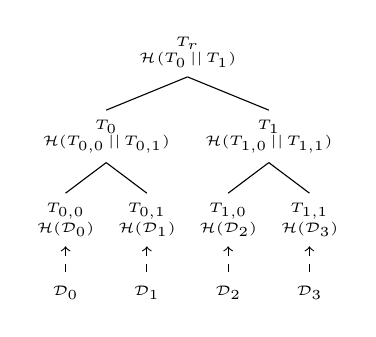
\begin{tikzpicture}
          \tikzset{every tree node/.style={align=center,anchor=north,font=\tiny}}
          \Tree
            [.\node{$T_{r}$ \\ $\hash{T_{0} \concat T_{1}}$};
              [.\node{$T_{0}$ \\ $\mathcal{H}(T_{0, 0} \concat T_{0, 1})$};
                [.{$T_{0, 0}$ \\ $\mathcal{H}(\mathcal{D}_{0})$}
                  \edge[dashed, style={<-}] node {}; $\mathcal{D}_{0}$
                ]
                [.{$T_{0, 1}$ \\ $\mathcal{H}(\mathcal{D}_{1})$}
                  \edge[dashed, style={<-}] node {}; $\mathcal{D}_{1}$
                ]
              ]
              [.\node{$T_{1}$ \\ $\mathcal{H}(T_{1, 0} \concat T_{1, 1})$};
                [.{$T_{1, 0}$ \\ $\mathcal{H}(\mathcal{D}_{2})$}
                  \edge[dashed, style={<-}] node {}; $\mathcal{D}_{2}$
                ]
                [.{$T_{1, 1}$ \\ $\mathcal{H}(\mathcal{D}_{3})$}
                  \edge[dashed, style={<-}] node {}; $\mathcal{D}_{3}$
                ]
              ]
            ]
        \end{tikzpicture}
        \captionsetup{font=scriptsize}
        \caption*{Take $\mathcal{D}_n$ as any data block. A Merkle tree
          can be constructed recursively through the concatenation
          of hashes of a node's children.}
      \end{figure}
    \end{column}
  \end{columns}
\end{frame}

\begin{frame}[plain,noframenumbering]
  \frametitle{Bibliography}
  \bibliographystyle{alpha}
  \bibliography{report}
\end{frame}

\end{document}
